% Copyright 2007 by Till Tantau
%
% This file may be distributed and/or modified
%
% 1. under the LaTeX Project Public License and/or
% 2. under the GNU Public License.
%
% See the file doc/licenses/LICENSE for more details.

\documentclass[portuguese,10pt,xcolor=table]{bredelebeamer}
\setbeameroption{show notes}
%\setbeamertemplate{note page}{Notas:\\\pagecolor{yellow!5}\insertnote}
%\usepackage{beamerthemeshadow}
%\usetheme{Berlin}
%\usecolortheme{lily}
%\usecolortheme{beaver}

\usepackage[brazil]{babel}
\usepackage[utf8]{inputenc}
\usepackage{times}
\usepackage{varwidth}
\usepackage{tikz}
\usepackage[tikz]{bclogo}
\usetikzlibrary{arrows,shapes}

\usetikzlibrary{calc,decorations.pathmorphing,patterns}
\pgfdeclaredecoration{penciline}{initial}{
	\state{initial}[width=+\pgfdecoratedinputsegmentremainingdistance,
		auto corner on length=1mm,]{
			\pgfpathcurveto%
			{% From
				\pgfqpoint{\pgfdecoratedinputsegmentremainingdistance}
				{\pgfdecorationsegmentamplitude}
			}
			{%  Control 1
				\pgfmathrand
					\pgfpointadd{\pgfqpoint{\pgfdecoratedinputsegmentremainingdistance}{0pt}}
				{\pgfqpoint{-\pgfdecorationsegmentaspect
							   \pgfdecoratedinputsegmentremainingdistance}%
							   {\pgfmathresult\pgfdecorationsegmentamplitude}
				}
			}
			{%TO 
				\pgfpointadd{\pgfpointdecoratedinputsegmentlast}{\pgfpoint{1pt}{1pt}}
			}
		}
	\state{final}{}
}



\everymath{\displaystyle}
\tikzstyle{every picture}+=[remember picture,decoration=penciline]
%\tikzstyle{every node}+=[decorate]
%\tikzstyle{every path}+=[decorate]
%\tikzstyle{na} = [baseline=-.5ex]

\usepackage[T1]{fontenc}

\def\lecturename{IMD0012 - Introdução às técnicas de programação}

\title{\insertlecture}

\author{Prof. Fernando Figueira\\(adaptado do material do Prof. Rafael Beserra Gomes)}

\institute{UFRN}

\subject{Introdução à disciplina de algoritmos, de forma sucinta: conceitos de algoritmos, sistemas computacionais e linguagens de programação}

\lecture[]{Introdução a algoritmos}{}

%\subtitle{subtitulo}

\date{}

\begin{document}

\usebackgroundtemplate{%
	
\includegraphics[width=\paperwidth,height=\paperheight]{background2}
}
\begin{frame}
  \maketitle
 \begin{center}
 \tiny
Material compilado em \today.
  Licença desta apresentação:\\
		
\includegraphics[height=1.0cm]{by-nc-nd.png}\\
http://creativecommons.org/licenses/
	\end{center}
\end{frame}

\section{Algoritmos}

\subsection{Conceitos iniciais de algoritmos}
	\begin{frame} 
		\begin{beamerboxesrounded}{Objetivo}
		Sequência ordenada e não ambígua de passos que levam à solução de um dado problema [TREMBLAY, 1979].
		\end{beamerboxesrounded}
	\end{frame}


	\begin{frame}
	\small
Exemplos:
\begin{itemize}
\item Como ir do IMD até o Natal Shopping?
\item Tarefas do studio.code.org
\end{itemize}


	\vspace{1cm}
		\begin{itemize}
		\item Quais são os passos possíveis no algoritmo?
		\item Existe um único algoritmo para finalizar cada etapa?
		\end{itemize}
	\end{frame}

\subsection{Algoritmos computacionais}

	\begin{frame}
		\begin{center}
			\structure{\Huge \insertsubsection}
		\end{center}
	\end{frame} 

	\begin{frame} 
		\begin{beamerboxesrounded}{Algoritmo computacional}
		Um algoritmo que pode ser traduzido em uma sequência de instruções que pode ser executado em um computador.
		\end{beamerboxesrounded}
	\end{frame}

	\begin{frame} 
		\begin{itemize}
		\item Os algoritmos serão expressos de acordo com o que o computador pode executar
		\item Vamos conhecer um pouco mais sobre o computador!
		\end{itemize}
	\end{frame}


\section{Sistemas computacionais}

	\begin{frame}
		\begin{center}
			\structure{\Huge \insertsection}
		\end{center}
	\end{frame} 

\subsection{Introdução}
\def \BLOCO {
	\node[shape=coordinate] (c1){teste};
	\node[shape=coordinate, below of=c1] (c2){teste};
	\node[shape=coordinate, below of=c2] (c3){teste};
	\node[shape=coordinate, below of=c3] (c4){teste};

	\node[style=bloco,right of=c1,anchor=west] (b1) {Adquire dados};
	\node[style=bloco,right of=c2,anchor=west] (b2) {Armazena dados};
	\node[style=bloco,right of=c3,anchor=west] (b3) {Processa dados};
	\node[style=bloco,right of=c4,anchor=west] (b4) {Exibe dados};

	\node[shape=coordinate, right of=b1] (c1){teste};
	\node[shape=coordinate, below of=c1] (c2){teste};
	\node[shape=coordinate, below of=c2] (c3){teste};
	\node[shape=coordinate, below of=c3] (c4){teste};
}

	\tikzstyle{bloco}=[inner sep=4pt,fill=blue!20,opacity=0.8,rounded corners,scale=1]
	\tikzstyle{explicabloco}=[inner sep=4pt,fill=blue!20,opacity=0.8,rounded corners,scale=0.82,align=left]

	\def\titulo{Sistema computacional}
	\begin{frame} 
	\begin{tikzpicture}
		\BLOCO
	\end{tikzpicture}
	\end{frame}

	\begin{frame} 
	\begin{tikzpicture}
		\BLOCO
		\node[style=explicabloco,right of=c1,anchor=west,right=20pt] (e1) {
			Obtemos informações do mundo\\através de \textbf{dispositivos de entrada}.
		};
		\path[->] (e1) edge [] (b1);
	\end{tikzpicture}
	\end{frame}
	\begin{frame} 
	\begin{tikzpicture}
		\BLOCO
		\node[style=explicabloco,right of=c1,anchor=west,right=20pt] (e1) {
			Obtemos informações do mundo\\através de \textbf{dispositivos de entrada}:\\
				- Teclado (texto)\\
				- Câmera (imagens)\\
				- Scanner (imagens)\\
				- Leitor de digitais (imagens)\\
				- Microfone (som)\\
				- Mouse (coordenada, botões)\\
				- Eletrocardiógrafo (atividade elétrica no coração)\\
				- Touch Screen
		};
		\path[->] (e1) edge [] (b1);
	\end{tikzpicture}
	\end{frame}

	\begin{frame}
	\begin{tikzpicture}
		\BLOCO
		\node[style=explicabloco,right of=c2,anchor=west,right=20pt] (e2) {
			Através das memórias é possível armazenar dados.
		};
		\path[->] (e2) edge [] (b2);
	\end{tikzpicture}
	\end{frame}

	\begin{frame}
	\begin{tikzpicture}
		\BLOCO
		\node[style=explicabloco,right of=c2,anchor=west,right=20pt] (e2) {
			Através das memórias é possível armazenar dados:\\\\
				\textbf{Memória volátil}\\
				Os dados são perdidos quando a energia cessa\\
				- Mem. RAM, mem. cache, registradores (memória principal)\\
				\textbf{Memória não volátil}\\
				- HD, cartão de memória, CD, DVD, Pen-Drive\\(memória secundária)\\
		};
		\path[->] (e2) edge [] (b2);
	\end{tikzpicture}
	\end{frame}

	\begin{frame}
	\begin{tikzpicture}
		\BLOCO
		\node[style=explicabloco,right of=c3,anchor=west,right=20pt] (e3) {
			O processamento dos dados é usualmente realizado\\
				por um ou mais processadores (CPU).\\
				O processador contém registradores e efetuam\\ nestes operações básicas como:\\
				adição, subtração, multiplicação.

		};
		\path[->] (e3) edge [] (b3);
	\end{tikzpicture}
	\end{frame}

	\begin{frame}
	\begin{tikzpicture}
		\BLOCO
		\node[style=explicabloco,right of=c4,anchor=west,right=20pt] (e4) {
			O computador utiliza \textbf{dispositivos de saída}\\
				para que esses dados sejam compreensíveis\\
				para o ser humano.
		};
		\path[->] (e4) edge [] (b4);
	\end{tikzpicture}
	\end{frame}

	\begin{frame}
	\begin{tikzpicture}
		\BLOCO
		\node[style=explicabloco,right of=c4,anchor=west,right=20pt] (e4) {
			O computador utiliza \textbf{dispositivos de saída}\\
				para que esses dados sejam compreensíveis\\
				para o ser humano:\\
				- Impressora\\
				- Monitor\\
				- Alto-falante
		};
		\path[->] (e4) edge [] (b4);
	\end{tikzpicture}
	\end{frame}

\subsection{Sistema operacional}
	\begin{frame} 
		\begin{beamerboxesrounded}{Sistema Operacional}
		O sistema operacional (SO) é um conjunto de softwares que controla os recursos do computador e oferece serviços básicos para qualquer aplicativo. Entre os sistemas operacionais mais conhecidos estão:
		\begin{itemize}
			\item Windows
			\item Linux (diversas distribuições como Ubuntu)
			\item Android (baseado em Linux)
			\item Mac OS
		\end{itemize}
		\end{beamerboxesrounded}
	\end{frame}


	\begin{frame} 
	\footnotesize
	\begin{beamerboxesrounded}{Programas}
		Programas (software) são sequência de instruções que podem ser executadas em um processador.
	\end{beamerboxesrounded}
\vspace{0.3cm}Exemplos:\\
		\tikz \node[align=left,anchor=west,inner sep=4pt,fill=blue!20,opacity=0.8,rounded corners,scale=0.82,align=left](e9){\footnotesize Processador de texto};
		\tikz \node[align=left,anchor=west,inner sep=4pt,fill=gray!20,opacity=0.8,rounded corners,scale=0.82,align=left](e9){\footnotesize Microsoft Word, OpenOffice Writer, Latex};\\
		
		\tikz \node[align=left,anchor=west,inner sep=4pt,fill=blue!20,opacity=0.8,rounded corners,scale=0.82,align=left](e9){\footnotesize Editor de imagens};
		\tikz \node[align=left,anchor=west,inner sep=4pt,fill=gray!20,opacity=0.8,rounded corners,scale=0.82,align=left](e9){\footnotesize Adobe Photoshop, Gimp};\\
		
		\tikz \node[align=left,anchor=west,inner sep=4pt,fill=blue!20,opacity=0.8,rounded corners,scale=0.82,align=left](e9){\footnotesize Editor de vídeos};
		\tikz \node[align=left,anchor=west,inner sep=4pt,fill=gray!20,opacity=0.8,rounded corners,scale=0.82,align=left](e9){\footnotesize Adobe After Effects, Sony Vegas};\\

		\tikz \node[align=left,anchor=west,inner sep=4pt,fill=blue!20,opacity=0.8,rounded corners,scale=0.82,align=left](e9){\footnotesize Científicos};
		\tikz \node[align=left,anchor=west,inner sep=4pt,fill=gray!20,opacity=0.8,rounded corners,scale=0.82,align=left](e9){\footnotesize Matlab, Geogebra};\\

		\tikz \node[align=left,anchor=west,inner sep=4pt,fill=blue!20,opacity=0.8,rounded corners,scale=0.82,align=left](e9){\footnotesize Jogos};
		\tikz \node[align=left,anchor=west,inner sep=4pt,fill=gray!20,opacity=0.8,rounded corners,scale=0.82,align=left](e9){\footnotesize Stunts, Sim City, Super Mario, Street Fighter};\\
		
		\tikz \node[align=left,anchor=west,inner sep=4pt,fill=blue!20,opacity=0.8,rounded corners,scale=0.82,align=left](e9){\footnotesize Animação};
		\tikz \node[align=left,anchor=west,inner sep=4pt,fill=gray!20,opacity=0.8,rounded corners,scale=0.82,align=left](e9){\footnotesize 3D Studio, Maya, Blender, Adobe Flash};\\
		
		\tikz \node[align=left,anchor=west,inner sep=4pt,fill=blue!20,opacity=0.8,rounded corners,scale=0.82,align=left](e9){\footnotesize Navegadores};
		\tikz \node[align=left,anchor=west,inner sep=4pt,fill=gray!20,opacity=0.8,rounded corners,scale=0.82,align=left](e9){\footnotesize Internet Explorer, Mozilla Firefox, Opera, Google Chrome};\\
		
		\tikz \node[align=left,anchor=west,inner sep=4pt,fill=blue!20,opacity=0.8,rounded corners,scale=0.82,align=left](e9){\footnotesize Programas mais simples};
		\tikz \node[align=left,anchor=west,inner sep=4pt,fill=gray!20,opacity=0.8,rounded corners,scale=0.82,align=left](e9){\footnotesize cat, calculadora, grep, head, ipconfig (ifconfig)};\\

		Você é capaz de responder com que tipo de informações cada programa desse trabalha?
	\end{frame}

\subsection{Memória}
	\def\GN[#1]{\colorbox{white!100}{#1}}
	\def\RN[#1]{\colorbox{white!100}{#1}}
	\def\BN[#1]{\colorbox{white!100}{#1}}
	\def\ON[#1]{\colorbox{white!100}{#1}}
	\def\WN[#1]{\colorbox{white!100}{#1}}
%	\def\GN[#1]{\colorbox{gray!40}{#1}}
%	\def\RN[#1]{\colorbox{red!40}{#1}}
%	\def\BN[#1]{\colorbox{blue!40}{#1}}
%	\def\ON[#1]{\colorbox{orange!40}{#1}}
%	\def\WN[#1]{\colorbox{white!40}{#1}}

	\begin{frame}
		\begin{center}
			\structure{\large Como essas informações são representadas em um computador?}
		\end{center}
	\end{frame} 

\def\titulo{Representação dos dados na memória}
	\begin{frame}
	Os dados na memória são armazenados em sequências de bits
		\tiny
		 \setlength{\tabcolsep}{0pt}	
		\begin{table}
				  \begin{tabular}{|c|c|c|c|c|c|c|c|c|c|c|c|c|c|c|c|c|c|c|c|c|c|c|c|c|c|c|c|c|c|c|c|}
					\hline
		 \WN[0]&\WN[1]&\WN[0]&\WN[0]&\WN[1]&\WN[1]&\WN[0]&\WN[0]& 
		 \RN[0]&\RN[1]&\RN[0]&\RN[0]&\RN[1]&\RN[1]&\RN[0]&\RN[0]& 
		 \WN[0]&\WN[1]&\WN[0]&\WN[0]&\WN[1]&\WN[1]&\WN[0]&\WN[0]& 
		 \WN[0]&\WN[1]&\WN[0]&\WN[0]&\WN[0]&\WN[0]&\WN[0]&\WN[0] \\\hline
				\end{tabular}
		\end{table}
		\tikz \node[align=left,anchor=west,inner sep=4pt,fill=blue!20,opacity=0.8,rounded corners,scale=0.82,align=left](e9){\footnotesize 8 bits = 1 byte};\\
		\tikz \node[align=left,anchor=west,inner sep=4pt,fill=blue!20,opacity=0.8,rounded corners,scale=0.82,align=left](e9){\footnotesize 1024 bytes = 1 kilobyte (kB)};\\
		\tikz \node[align=left,anchor=west,inner sep=4pt,fill=blue!20,opacity=0.8,rounded corners,scale=0.82,align=left](e9){\footnotesize 1024 kilobytes = 1 megabyte (MB)};\\
		\tikz \node[align=left,anchor=west,inner sep=4pt,fill=blue!20,opacity=0.8,rounded corners,scale=0.82,align=left](e9){\footnotesize 1024 megabytes = 1 gigabyte (GB)};
	\end{frame}

	\begin{frame}
	Um tipo de dado corresponde a uma sequência de bits de tamanho fixo com uma interpretação específica.\\\vspace{0.3cm}
		\tikz \node[align=left,anchor=west,inner sep=4pt,fill=blue!20,opacity=0.8,rounded corners,scale=0.82,align=left](e9){\footnotesize número inteiro = 4 bytes};

		\tikz \node[align=left,anchor=west,inner sep=4pt,fill=blue!20,opacity=0.8,rounded corners,scale=0.82,align=left](e9){\footnotesize número real = 4 bytes};
		\tikz \node[align=left,anchor=west,inner sep=4pt,fill=gray!20,opacity=0.8,rounded corners,scale=0.82,align=left](e9){\footnotesize padrão IEEE 754};\\

		\tikz \node[align=left,anchor=west,inner sep=4pt,fill=blue!20,opacity=0.8,rounded corners,scale=0.82,align=left](e9){\footnotesize um caractere ASCII = 1 byte};
		\tikz \node[align=left,anchor=west,inner sep=4pt,fill=gray!20,opacity=0.8,rounded corners,scale=0.82,align=left](e9){\footnotesize por exemplo: A = 65 (01000001)};\\

		\tikz \node[align=left,anchor=west,inner sep=4pt,fill=blue!20,opacity=0.8,rounded corners,scale=0.82,align=left](e9){\footnotesize um caractere Unicode = 4 bytes};
		\tikz \node[align=left,anchor=west,inner sep=4pt,fill=gray!20,opacity=0.8,rounded corners,scale=0.82,align=left](e9){\footnotesize cerca de 107 mil caracteres};\\
		\note[item]{No Linux você pode conferir a tabela ASCII digitando \textbf{man ascii} (q para sair do manual). Sempre que houver alguma dúvida sobre algum comando do Linux, você pode tentar consultar o manual. Por exemplo, para ver o manual do ls: \textbf{man ls}}
	\end{frame}

	\subsubsection{Imagens e sons}
	\begin{frame}

	\begin{beamerboxesrounded}{Imagem}
	\footnotesize Uma imagem digital é composta por pixels.
	\end{beamerboxesrounded}
		\tikz \node[opacity=1.0](fig1){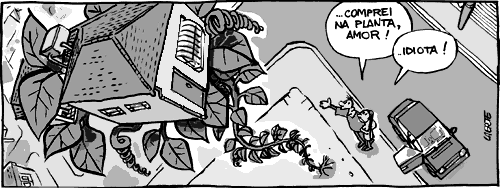
\includegraphics[width=200px]{plantaCinza.png}};
		\tikz \node[overlay,left of=fig1,draw,fill=white,opacity=0.8,right=1.04cm,above=0.4cm,minimum width=11pt, minimum height=11pt](figSelecao){ };
		\tikz \node[](fig2){
\includegraphics[width=50px]{plantaZoomEscalaCinza.png}};
		\tikz[overlay] \path[decorate,->] (figSelecao.east) edge[line width=2pt, red, bend right, dotted] (fig2.west);\\
		
		\tikz \node[](fig2){
\includegraphics[width=300px]{escalaCinza.png}};\\\vspace{0.5cm}
		\tikz \node[](preto){\footnotesize Preto (valor 0)};\hspace{2.1cm}
		\tikz \node[](cinza){\footnotesize Cinza (valor 127)};\hspace{1.3cm}
		\tikz \node[](branco){\footnotesize Branco (valor 255)};
		\tikz[overlay] \path[decorate,->] (preto.west) edge[line width=1pt, bend left, dotted] (fig2.west);\\
		\tikz[overlay] \path[decorate,->] (cinza.north) edge[line width=1pt, dotted] (fig2.south);\\
		\tikz[overlay] \path[decorate,->] (branco.east) edge[line width=1pt, bend right, dotted] (fig2.east);\\
	\end{frame}

	\begin{frame}
	\begin{beamerboxesrounded}{Imagem colorida}
	\footnotesize Em uma imagem colorida, cada pixel pode ser descrito como a composição de 3 canais: R (red) , G (green), B (blue)
	\end{beamerboxesrounded}
		\tikz \node[opacity=1.0](fig1){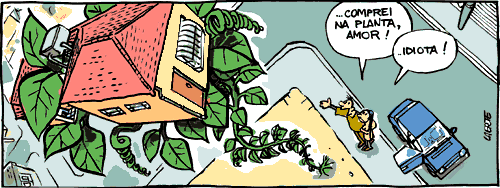
\includegraphics[width=200px]{planta.png}};
		\tikz \node[overlay,left of=fig1,draw,fill=white,opacity=0.8,right=1.04cm,above=0.4cm,minimum width=11pt, minimum height=11pt](figSelecao){ };
		\tikz \node[](fig2){
\includegraphics[width=50px]{plantaZoomColorido.png}};
		\tikz[overlay] \path[decorate,->] (figSelecao.east) edge[line width=2pt, red, bend right, dotted] (fig2.west);\\
		
		\tikz \node[](fig2){
\includegraphics[width=50px]{corVerde.png}};\\
		\tikz \node[](fig2){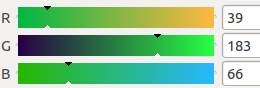
\includegraphics[width=100px]{escalaRgb.png}};
		\tikz[overlay] \node[right of=fig2,right=2cm,above=0.5cm,anchor=west](preto){\footnotesize Componente vermelho};
		\tikz[overlay] \node[right of=fig2,right=2cm,anchor=west](cinza){\footnotesize Componente verde};
		\tikz[overlay] \node[right of=fig2,right=2cm,below=0.5cm,anchor=west](branco){\footnotesize Componente azul};
		\tikz[overlay] \path[decorate,->] (preto.west) edge[line width=1pt, bend right, dotted] (fig2.east |- preto.west);
		\tikz[overlay] \path[decorate,->] (cinza.west) edge[line width=1pt, dotted] (fig2.east);
		\tikz[overlay] \path[decorate,->] (branco.west) edge[line width=1pt, bend left, dotted] (fig2.east |- branco.west);
	\end{frame}

	\begin{frame}
		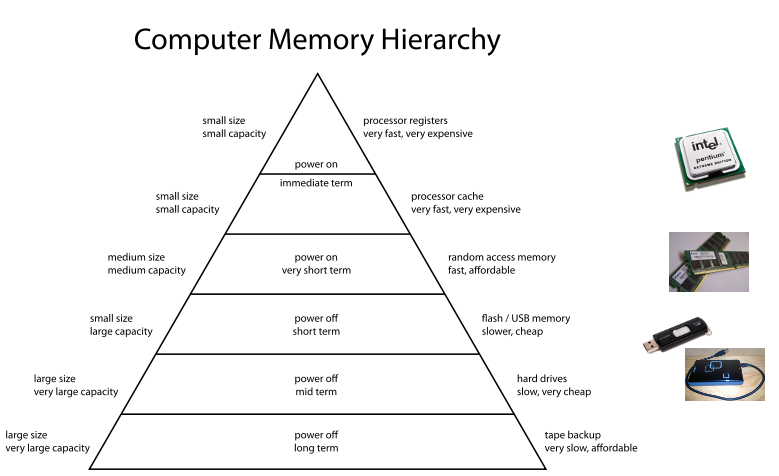
\includegraphics[width=11cm]{memoria2.png}
		\note[item]{Note que quanto mais rápida a memória, mais cara. Por esse motivo, as memórias mais rápidas também possuem menor capacidade de armazenamento.}
	\end{frame}


	\subsection{CPU}

	%definir clock, registradores
	\def\BA{A CPU (unidade central de processamento) é \\ um dos responsáveis pelo processamento\\dos dados em um computador.}
	\def\BB{A cada ciclo de clock uma\\instrução é executada na CPU.}
	\def\BC{O conjunto de instruções disponível\\depende do modelo de processador.}

	\def\titulo{A CPU}
	\tikzstyle{blocoLigado}=[anchor=west,inner sep=4pt,fill=blue!20,opacity=0.8,rounded corners=10pt,scale=0.72,minimum height=90pt,align=left]
	\tikzstyle{blocoDesligado}=[anchor=west,inner sep=4pt,fill=blue!20,opacity=0.14,rounded corners=10pt,scale=0.72,minimum height=90pt,align=left]

	\begin{frame}
		\tikz \node[style=blocoLigado](e9){\BA};
		\tikz \node[style=blocoDesligado](e9){\BB};
		\tikz \node[style=blocoDesligado](e9){\BC};
		\tikz \node[](e9){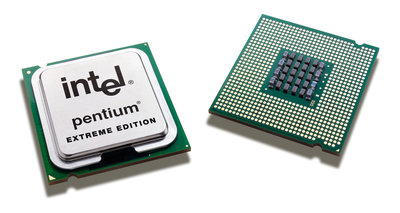
\includegraphics[height=60pt]{processador.png}};
	\end{frame}
	\begin{frame}
		\tikz \node[style=blocoDesligado](e9){\BA};
		\tikz \node[style=blocoLigado](e9){\BB};
		\tikz \node[style=blocoDesligado](e9){\BC};
		\tikz \node[](e9){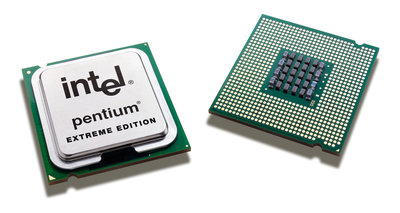
\includegraphics[height=60pt]{processador.png}};
	\end{frame}
	\begin{frame}
		\tikz \node[style=blocoDesligado](e9){\BA};
		\tikz \node[style=blocoDesligado](e9){\BB};
		\tikz \node[style=blocoLigado](e4){\BC};
		\tikz \node[opacity=0.1](e5){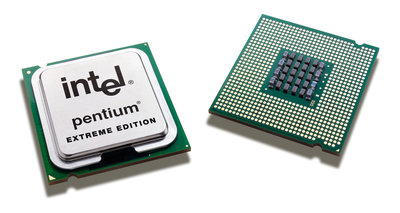
\includegraphics[height=60pt]{processador.png}};
%\ECFAugie 
		\tikz[overlay] \node[anchor=west,right of=e4,right=70pt,align=left,inner sep=4pt,fill=red!20,opacity=0.8,rounded corners,scale=0.82,align=left](e9){Instruções básicas como:\\- somar valores de dois endereços\\- multiplicar dois números\\- obter um valor da memória};
		\tikz[overlay] \path[decorate,->] (e9.west) edge[decorate] (e4.east);
		
	\end{frame}

	\begin{frame} 
%		Na linguagem Assembly cada instrução corresponde a uma instrução de máquina.
		Quais são as instruções disponíveis para criar algoritmos no computador?\\
		\textbf{Linguagem/código de máquina}
		\begin{itemize}
			\item Específica para cada arquitetura de computador
			\item Um exemplo fictício (processador de 16 bits):
		\tiny
		 \setlength{\tabcolsep}{0pt}
		\begin{table}
			\begin{center}
				  \begin{tabular}{|c|c|c|c|c|c|c|c|c|c|c|c|c|c|c|c|}
					\hline
					\colorbox{red!40}{0} & 
					\colorbox{red!40}{0} & 
					\colorbox{red!40}{0} & 
					\colorbox{red!40}{0} & 
					\colorbox{red!40}{0} & 
					\colorbox{gray!40}{0} & 
					\colorbox{gray!40}{0} & 
					\colorbox{gray!40}{0} & 
					\colorbox{blue!40}{0} & 
					\colorbox{blue!40}{0} & 
					\colorbox{blue!40}{1} & 
					\colorbox{blue!40}{0} & 
					\colorbox{blue!40}{0} & 
					\colorbox{blue!40}{0} & 
					\colorbox{blue!40}{0} & 
					\colorbox{blue!40}{0} \\
						\hline
				  \end{tabular}
			\end{center}
		\end{table}
		\normalsize
		\begin{itemize}
			\item 5 bits: instrução
			\item 3 bits: registrador
			\item 8 bits: valor
		\end{itemize}
		\item Por exemplo: 10110 é o código para colocar um valor em um determinado registrador. Os 3 seguintes bits especificam qual registrador. Os demais 8 bits representam o valor a ser armazenado no registrador.
		\end{itemize}
	\end{frame}

	\begin{frame}
\begin{itemize}
\item Quer saber como funciona o seu processador e o conjunto de instruções? Leia o manual! https://software.intel.com/en-us/articles/intel-sdm
\item Programar em linguagem de máquina é um trabalho árduo
\item A \textbf{linguagem assembly} utiliza uma linguagem mais fácil para escrever programas
\item Um \textit{assembler} transforma um código em \textit{assembly} para código de máquina
\end{itemize}
		\note[item]{Não vamos programar em linguagem de máquina nessa disciplina.}
		\note[item]{A memória principal armazena tanto dados do programa como os próprios programas}
		\note[item]{Geralmente o HD faz o papel de memória secundária. Geralmente os programas estão armazenados nessa memória, mas quando solicitamos sua execução, as instruções são transferidas para a memória principal (memória RAM).}
	\end{frame}

%=======================================================================
%=======================================================================
\section{Linguagens de Programação}
	\begin{frame}
		\begin{center}
			\structure{\Huge \insertsection}
		\end{center}
	\end{frame} 

	\subsection{Conceitos}
	\begin{frame}
	\footnotesize
	As \colorbox{blue!30}{linguagens de programação} facilitam a programação de computadores. \\

	\end{frame}

%=======================================================================
%=======================================================================

	\begin{frame}
		\tikz \path node [anchor=west,inner sep=4pt,fill=gray!20,opacity=0.8,scale=0.82,draw](e9){\footnotesize C++};
		\tikz \path node [anchor=west,inner sep=4pt,fill=gray!20,opacity=0.8,scale=0.82,draw](e9){\footnotesize Pascal};
		\tikz \path node  [anchor=west,inner sep=4pt,fill=gray!20,opacity=0.8,scale=0.82,draw](e9){\footnotesize Portugol};
		\tikz \path node [anchor=west,inner sep=4pt,fill=gray!20,opacity=0.8,scale=0.82,draw](e9){\footnotesize Java};
		\tikz \path node  [anchor=west,inner sep=4pt,fill=gray!20,opacity=0.8,scale=0.82,draw](e9){\footnotesize C};
		\tikz \path node [anchor=west,inner sep=4pt,fill=gray!20,opacity=0.8,scale=0.82,draw](e9){\footnotesize Python};
		\tikz \path node [anchor=west,inner sep=4pt,fill=gray!20,opacity=0.8,scale=0.82,draw](e9){\footnotesize Ruby};
		\tikz \path node  [anchor=west,inner sep=4pt,fill=gray!20,opacity=0.8,scale=0.82,draw](e9){\footnotesize Basic};
		\tikz \path node [anchor=west,inner sep=4pt,fill=gray!20,opacity=0.8,scale=0.82,draw](e9){\footnotesize Matlab};
		\tikz \path node  [anchor=west,inner sep=4pt,fill=gray!20,opacity=0.8,scale=0.82,draw](e9){\footnotesize Lua};
		\tikz \path node  [anchor=west,inner sep=4pt,fill=gray!20,opacity=0.8,scale=0.82,draw](e9){\footnotesize JavaScript};
		\tikz \path node  [anchor=west,inner sep=4pt,fill=gray!20,opacity=0.8,scale=0.82,draw](e9){\footnotesize Perl};
		\tikz \path node  [anchor=west,inner sep=4pt,fill=gray!20,opacity=0.8,scale=0.82,draw](e9){\footnotesize PHP};
		\tikz \path node  [anchor=west,inner sep=4pt,fill=gray!20,opacity=0.8,scale=0.82,draw](e9){\footnotesize Lisp};
		\tikz \path node  [anchor=west,inner sep=4pt,fill=gray!20,opacity=0.8,scale=0.82,draw](e9){\footnotesize C\#};
		\tikz \path node  [anchor=west,inner sep=4pt,fill=gray!20,opacity=0.8,scale=0.82,draw](e9){\footnotesize Fortran};
		\tikz \path node  [anchor=west,inner sep=4pt,fill=gray!20,opacity=0.8,scale=0.82,draw](e9){\footnotesize Scheme};
		\tikz \path node  [anchor=west,inner sep=4pt,fill=gray!20,opacity=0.8,scale=0.82,draw](e9){\footnotesize Haskell};
	\end{frame}
	\begin{frame}
		\tikz \path node [anchor=west,inner sep=4pt,fill=gray!20,opacity=0.2,scale=0.82,draw](e9){\footnotesize C++};
		\tikz \path node [anchor=west,inner sep=4pt,fill=gray!20,opacity=0.2,scale=0.82,draw](e9){\footnotesize Pascal};
		\tikz \path node  [anchor=west,inner sep=4pt,fill=gray!20,opacity=0.2,scale=0.82,draw](e9){\footnotesize Portugol};
		\tikz \path node [anchor=west,inner sep=4pt,fill=gray!20,opacity=0.2,scale=0.82,draw](e9){\footnotesize Java};
		\tikz \path node  [anchor=west,inner sep=4pt,fill=gray!20,opacity=0.8,scale=0.82,draw](eP){\footnotesize C};
		\tikz \path node [anchor=west,inner sep=4pt,fill=gray!20,opacity=0.2,scale=0.82,draw](e9){\footnotesize Python};
		\tikz \path node [anchor=west,inner sep=4pt,fill=gray!20,opacity=0.2,scale=0.82,draw](e9){\footnotesize Ruby};
		\tikz \path node  [anchor=west,inner sep=4pt,fill=gray!20,opacity=0.2,scale=0.82,draw](e9){\footnotesize Basic};
		\tikz \path node [anchor=west,inner sep=4pt,fill=gray!20,opacity=0.2,scale=0.82,draw](e9){\footnotesize Matlab};
		\tikz \path node  [anchor=west,inner sep=4pt,fill=gray!20,opacity=0.2,scale=0.82,draw](e9){\footnotesize Lua};
		\tikz \path node  [anchor=west,inner sep=4pt,fill=gray!20,opacity=0.2,scale=0.82,draw](e9){\footnotesize JavaScript};
		\tikz \path node  [anchor=west,inner sep=4pt,fill=gray!20,opacity=0.2,scale=0.82,draw](e9){\footnotesize Perl};
		\tikz \path node  [anchor=west,inner sep=4pt,fill=gray!20,opacity=0.2,scale=0.82,draw](e9){\footnotesize PHP};
		\tikz \path node  [anchor=west,inner sep=4pt,fill=gray!20,opacity=0.2,scale=0.82,draw](e9){\footnotesize Lisp};
		\tikz \path node  [anchor=west,inner sep=4pt,fill=gray!20,opacity=0.2,scale=0.82,draw](e9){\footnotesize C\#};
		\tikz \path node  [anchor=west,inner sep=4pt,fill=gray!20,opacity=0.2,scale=0.82,draw](e9){\footnotesize Fortran};
		\tikz \path node  [anchor=west,inner sep=4pt,fill=gray!20,opacity=0.2,scale=0.82,draw](e9){\footnotesize Scheme};
		\tikz \path node  [anchor=west,inner sep=4pt,fill=gray!20,opacity=0.2,scale=0.82,draw](e9){\footnotesize Haskell};\\
\vspace{1.0cm}
		\tikz[] \node[align=left,anchor=west,inner sep=4pt,fill=blue!20,opacity=0.8,rounded corners,scale=0.82,align=left](e9){\footnotesize C é uma linguagem compilada};
		\tikz[overlay] \path[->] (e9.north) edge (eP.south);
		\note[item]{Cada linguagem de programação possui suas vantagens e desvantagens e, portanto, a linguagem mais indicada depende do contexto da aplicação.}
		\note[item]{A linguagem C apesar de bastante antiga é ainda uma das mais populares e é excelente para aprender programação.}
	\end{frame}

	\subsection{Sintaxe e semântica}
	\begin{frame}
	\begin{itemize}
		\item As linguagens de programação possuem regras de sintaxe e semântica!
		\item Um algoritmo escrito nessa linguagem de programação só será aceito se estiver completamente de acordo com as regras gramaticais
		
	\end{itemize}
	\end{frame}

	\subsection{Linguagens compiladas e interpretadas}
	\begin{frame}
	\footnotesize
	Nas \textbf{linguagens compiladas}, programas específicos chamados compiladores convertem um código escrito em uma linguagem (código-fonte) para uma sequência de instruções do processador.

	\begin{center}
	\begin{tikzpicture}
		\tikzstyle{bloco}=[inner sep=4pt,fill=blue!20,opacity=0.8,rounded corners,scale=0.8]
		\tikzstyle{explicabloco}=[inner sep=4pt,fill=blue!20,opacity=0.8,rounded corners,scale=0.82,align=left]
		\path node [style=bloco,anchor=east,fill=gray!10,draw] (b1) {Código-fonte};
		\path (b1.east)+(0.4,0) node [draw,style=bloco,fill=orange!30,anchor=west,minimum height=50pt,minimum width=90pt] (b2) {Compilador};
		\path (b2.east)+(0.4,0) node [style=bloco,fill=gray!10,anchor=west,draw] (b3) {Programa (executável)};
		\path[->] (b1.east |- b2.west) edge [] (b2.west);
		\path[->] (b2.east |- b3.west) edge [] (b3.west);
	\end{tikzpicture}
	\end{center}
	
	Nas \textbf{linguagens interpretadas}, um programa interpretador interpreta um código escrito em uma linguagem e executa a sequência de instruções correspondentes.
	\note[item]{As linguagens interpretadas tendem a ser mais lentas pois várias instruções são executadas com a finalidade de interpretar o código-fonte durante a execução do programa.}
	\note[item]{As linguagens interpretadas têm a grande vantagem de facilitar a portabilidade entre sistemas diferentes.}

	\begin{center}
	\begin{tikzpicture}
		\tikzstyle{bloco}=[inner sep=4pt,fill=blue!20,opacity=0.8,rounded corners,scale=0.8]
		\tikzstyle{explicabloco}=[inner sep=4pt,fill=blue!20,opacity=0.8,rounded corners,scale=0.82,align=left]
		\path node [style=bloco,anchor=east,fill=gray!10,draw] (b1) {Código-fonte};
		\path (b1.east)+(0.4,0) node [draw,style=bloco,fill=orange!30,anchor=west,minimum height=50pt,minimum width=90pt] (b2) {Interpretador};
		\path[->] (b1.east |- b2.west) edge [] (b2.west);
	\end{tikzpicture}
	\end{center}
	\end{frame}

	\begin{frame} 
	\small
	Neste curso utilizaremos como dispositivo de entrada um teclado e como dispositivo de saída o monitor através de um terminal do sistema em modo texto.\\
\vspace{0.5cm}
	Dispositivo de entrada:
		\tikz \node[align=left,anchor=west,inner sep=4pt,fill=gray!20,opacity=0.8,rounded corners,scale=0.82,draw,align=left](e9){\footnotesize Teclado};
		\tikz \node[align=left,anchor=west,inner sep=4pt,fill=gray!20,opacity=0.3,rounded corners,scale=0.82,align=left](e9){\footnotesize Scanner};
		\tikz \node[align=left,anchor=west,inner sep=4pt,fill=gray!20,opacity=0.3,rounded corners,scale=0.82,align=left](e9){\footnotesize Câmera};
		\tikz \node[align=left,anchor=west,inner sep=4pt,fill=gray!20,opacity=0.3,rounded corners,scale=0.82,align=left](e9){\footnotesize Mouse};
	\\	
	Dispositivo de saída:
		\tikz \node[align=left,anchor=west,inner sep=4pt,fill=gray!20,opacity=0.8,rounded corners,scale=0.82,draw,align=left](e9){\footnotesize Monitor (terminal)};
		\tikz \node[align=left,anchor=west,inner sep=4pt,fill=gray!20,opacity=0.3,rounded corners,scale=0.82,align=left](e9){\footnotesize Impressora};
		\tikz \node[align=left,anchor=west,inner sep=4pt,fill=gray!20,opacity=0.3,rounded corners,scale=0.82,align=left](e9){\footnotesize Alto-falante};
	
	\end{frame}

\subsection{Entrada e saída de um programa}
	\begin{frame}
	\footnotesize
	Cada programa a ser desenvolvido nesse curso terá uma \textbf{entrada} fornecido pelo usuário através do teclado e uma \textbf{saída} visualizável no monitor.

	\begin{center}
	\begin{tikzpicture}
		\tikzstyle{bloco}=[inner sep=4pt,fill=blue!20,opacity=0.8,rounded corners,scale=0.8]
		\tikzstyle{explicabloco}=[inner sep=4pt,fill=blue!20,opacity=0.8,rounded corners,scale=0.82,align=left]
		\path node [style=bloco,anchor=east,fill=gray!10,draw] (b1) {Entrada};
		\path (b1.east)+(0.4,0) node [draw,style=bloco,fill=orange!30,anchor=west,minimum height=50pt,minimum width=90pt] (b2) {Programa};
		\path (b2.east)+(0.4,0) node [style=bloco,fill=gray!10,anchor=west,draw] (b3) {Saída};
		\path[->] (b1.east |- b2.west) edge [] (b2.west);
		\path[->] (b2.east |- b3.west) edge [] (b3.west);
	\end{tikzpicture}
	\end{center}

Exemplo:\\

		\tikz \node[align=left,anchor=west,inner sep=4pt,fill=gray!20,opacity=0.8,rounded corners,scale=0.82,align=left](e9){
	Um programa que calcula a média de um aluno dadas as notas das 3 unidades:\\
		\textbf{Entrada}: nota 1, nota 2 e nota 3 (números reais)\\
		\textbf{Saída}: média parcial (número real)};

	\end{frame}

\section{Representação dos algoritmos}

	\begin{frame}
		\begin{center}
			\structure{\Huge \insertsection}
		\end{center}
	\end{frame} 
\begin{frame}
	Formas para representar um algoritmo:
	\begin{itemize}
		\item Narrativa (linguagem natural)
		\item Fluxograma
		\item Pseudo-código
	\end{itemize}

\end{frame}


\subsection{Narrativa}
\begin{frame}
	Narrativa:
\begin{itemize}
	\item Descrição textual em linguagem natural
	\item Útil para ideias iniciais (lembre-se de que o objetivo é ter um algoritmo escrito em uma linguagem de programação)
	\item Problema: determine se um número inteiro n maior que 0 é primo
		\item Solução 1: o número n é primo se ele é diferente de 1 e divisível somente por 1 e por ele próprio
		\item Solução 2: desconsiderando os casos triviais n = 1 e n = 2, verifique se há algum número entre 2 e n-1 que divide n. Se não houver, então é primo!
\end{itemize}
\end{frame}


\subsection{Fluxograma}
\begin{frame}
	Fluxograma
	\begin{itemize}
		\item Representação gráfica muito boa para visualizar o fluxo lógico
	\end{itemize}
	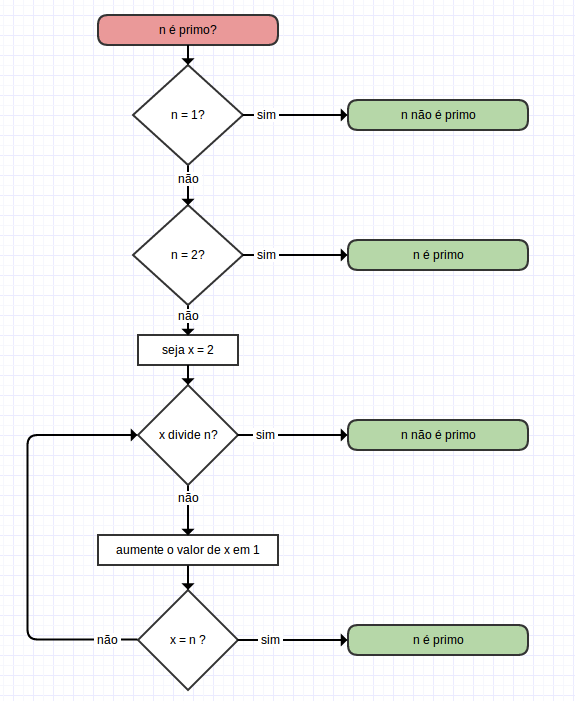
\includegraphics[height=7cm]{fluxograma.png}
	\note[item]{A representação em fluxograma não é muito comum, pois ocupa muito espaço e é difícil produzí-la.}
\end{frame}


\subsection{Pseudo-código}
\begin{frame}

	Pseudo-código
\begin{itemize}
	\item Representação mais próxima de uma linguagem de programação
	\item Flexibilidade em relação às regras gramaticais da linguagem e uso de linguagem natural
\end{itemize}
	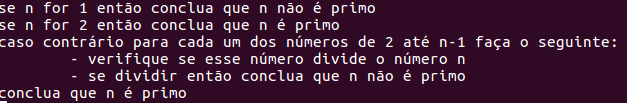
\includegraphics[height=1.5cm]{pseudocodigo.png}
\end{frame}

	
\end{document}

